\chapter{Methodology}
\label{chap:03}
\paragraph{}

The chapter provided a methodology  to discuss the involvement of the intracellular signalling network composed of STAT1, STAT3, Bcl-2, and BAX in regulating critical cellular states, including both anti-apoptosis and apoptosis of cancer cells, using Mathematical modeling. 
STAT1 plays a critical role in the control of T-cell homeostasis, and its suppressive/promoting role in tumorigenesis is influenced by environmental signals that might favour STAT1 activation in tumour cells or in host immune cells, respectively, with opposite consequences on tumour development. Interestingly, a mathematical framework will be adopted  to investigate how the STAT signalling pathways in cancer development and optimal control approaches can be modelled mathematically. And how intracellular module (STAT1, STAT3, Bcl-2 and BAX) dynamics play a key role in apoptotic cell death will be proved by using by illustrated results. This work will go over the intracellular module (STAT1, STAT3, Bcl-2 and BAX) ODEs system involving various situations and how they behave with different parameter values, as well as complex analysis using the Runge Kutta fourth order method and Euler's method and how to obtain the numerical analysis using software Java. Overall, these sources suggest that a mathematical approach is helpful in understanding the intracellular signalling network composed of STAT1, STAT3, Bcl-2, and BAX and its potential to be targeted for cancer therapy.


\newpage

\section{Biological approach of STAT1, STAT3, Bcl-2 and BAX}
\paragraph{}

The intracellular module (STAT1, STAT3, Bcl-2, and BAX) is a group of proteins that regulate various cellular processes, including cell growth, survival, and death. One approach to target these proteins is through the use of biologicals, such as drugs or other compounds that interact with these proteins to modulate their activity. One example of this is the use of niclosamide as a radiosensitizer in triple-negative breast cancer (TNBC) cells. Niclosamide was found to act by inhibiting STAT3 and Bcl-2 and increasing the generation of reactive oxygen species (ROS) in TNBC cells and xenograft tumours, leading to increased sensitivity to radiation therapy \cite{lu2018activation}. 

A mathematical model of STAT signalling pathways in cancer development and optimal control approaches was presented by Jonggul Lee, Donggu Lee 2 and Yangjin Kim in paper \cite{lee2021mathematical}. This model can be used to identify the potential targets for the biological approach in the treatment of cancer. It is worth mentioning that these proteins are complex and may have different effects in different contexts and cell types, so the biological approach should be tailored to the specific type of cancer and the stage of the disease. 

 \begin{figure}[hbt!]
	\centering
	\begin{framed}
	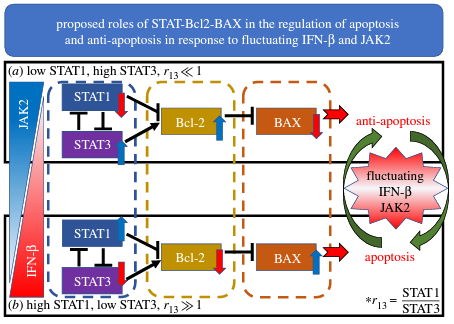
\includegraphics[width=0.75\textwidth]{Figures/stat.PNG}
		\end{framed}
	\caption{A schematic diagram for a proposed apoptosis signalling network in the presence of $IFN-\beta/JAK2$.\cite{lee2021mathematical}.}
	\label{fig:6}
\end{figure}

 
\subsection{Intracellular module of Signal Transducer and Activator of Transcription 1 (STAT1)}
\paragraph{}

The intracellular module of Signal Transducer and Activator of Transcription 1 (STAT1) is a protein that plays a key role in the body's immune response to viral infections. When activated, STAT1 binds to specific DNA sequences in the cell's genome, activating genes involved in the antiviral response. This includes the production of interferons and other cytokines, which help prevent the virus's spread throughout the body \cite{yang2021integrated}. Additionally, STAT1 can also inhibit the replication of certain viruses by blocking the activity of viral proteins. The intracellular module of STAT1 is activated by a variety of signalling pathways, including the Janus kinase (JAK) and phosphoinositide 3-kinase (PI3K) pathways. Dysregulation of STAT1 has been linked to a number of diseases, including cancer and autoimmune disorders. 

\subsection{Intracellular module of Signal Transducer and Activator of Transcription 3 (STAT3)}
\paragraph{}

The intracellular module of Signal Transducer and Activator of Transcription 3 (STAT3) is a protein that plays a key role in a variety of cellular processes, including cell growth, survival, and differentiation. According to the Human Protein Atlas project, the official gene symbol for STAT3 is "STAT3" \cite{stat3}, and the full gene name is "Signal transducer and activator of transcription 3". When activated, STAT3 binds to specific DNA sequences in the cell's genome, activating genes involved in cell growth, survival, and differentiation. It also plays a role in the inflammatory response, cell proliferation and differentiation. Also, when activated by certain cytokines, such as IL-11, IL-10, LIF, Oncostatin M and Leptin, STAT3 can enhance the Fas-mediated apoptosis of specific cells without any increase in cell surface Fas antigen expression \cite{tanaka2011stat3}. Furthermore, STAT3 siRNA transfection can suppress STAT3 expression and inhibit Fas-mediated cell death. [3] Dysregulation of STAT3 has been linked to a number of diseases, including cancer, autoimmune disorders, and others.

\subsection{Intracellular module of B-cell lymphoma 2 (Bcl-2)}
\paragraph{}

The intracellular module of B-cell lymphoma 2 (Bcl-2) is a family of proteins that play a key role in regulating the activation of the cell death program, also known as apoptosis. Some members of this family, like Bcl-2 itself or Bcl-XL, inhibit apoptosis by blocking the release of cytochrome c from mitochondria \cite{alberts2002programmed}. Bcl-2 proteins have been found in early metazoans including Porifera (sponges), Placozoans, and Cnidarians. Some viruses have gained Bcl-2 homologs and subvert innate immunity and cellular apoptosis for their replication, but they frequently have very different sequences to their host Bcl-2 analogues \cite{banjara2020bcl}. Intracellular flow cytometry can be used to measure the quantitative BCL-2 family protein abundance as a function of time and treatment to evaluate the mechanism(s) responsible for apoptotic triggering. Dysregulation of Bcl-2 family proteins has been linked to a number of diseases, including cancer, autoimmune disorders and others.

\subsection{Intracellular module of BCL-2-associated X protein (BAX)}
\paragraph{}

The intracellular module of BCL-2-associated X protein (BAX) is a protein that plays a key role in the regulation of the cell death program, also known as apoptosis. BAX is a member of the Bcl-2 family of proteins that promote apoptosis, in contrast to other members, such as Bcl-2 and Bcl-XL, which inhibit apoptosis. When BAX is activated, it oligomerizes and translocates to the mitochondria, where it can permeabilize the outer mitochondrial membrane and release pro-apoptotic factors such as cytochrome c \cite{andreu2017bax}. This leads to caspase activation, ultimately leading to cell degradation and death. BAX is activated by various signalling pathways, including the intrinsic and extrinsic pathways of apoptosis, and is regulated by other members of the Bcl-2 family, such as Bcl-2 and Bcl-XL. Dysregulation of BAX has been linked to a number of diseases, including cancer and neurodegenerative disorders \cite{czabotar2014control}. It's important to note that BAX is one of the vital proteins that initiate the cascade of events that leads to cell death via Apoptosis. It is a pro-apoptotic member of the Bcl-2 family of proteins, and its activation leads to the release of Cytochrome c from mitochondria, ultimately activating the cascade of caspases which leads to cell death.





\section{Mathematical model for intracellular module (STAT1, STAT3, Bcl-2 and BAX)}

\paragraph{}
The section should describe the mathematical models and techniques used to investigate the intracellular signalling network in more detail. First, a schematic diagram of the apoptosis signalling network will be described.   Key signalling network of apoptosis involving STAT1, STAT3, Bcl-2 and BAX in response to IFN-$\beta$ and JAK2 and the corresponding mathematical model: levels of STAT1 and STAT3 and activity of their target Bcl2 and BAX will be represented in more detail. 

\subsection{A schematic diagram of the apoptosis signalling network }
\paragraph{}

 \begin{figure}[hbt!]
	\centering
	\begin{framed}
	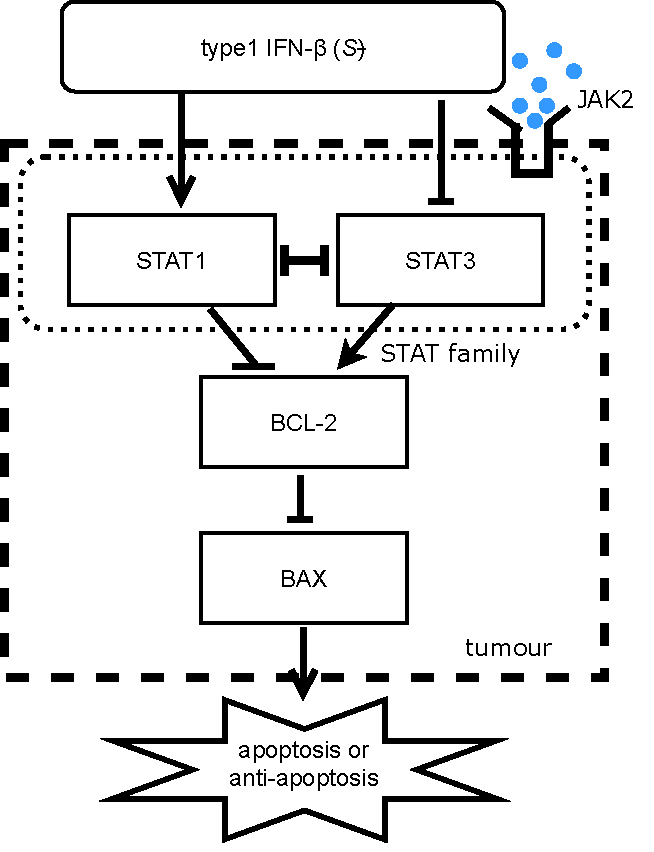
\includegraphics[width=0.7\textwidth]{Figures/D1.pdf}
		\end{framed}
	\caption{Key signalling network of apoptosis involving
STAT1, STAT3, Bcl-2 and BAX in response to IFN- $\beta$ and  JAK2  \cite{lee2021mathematical}.}
	\label{D1}
\end{figure}

 \begin{figure}[hbt!]
	\centering
	\begin{framed}
	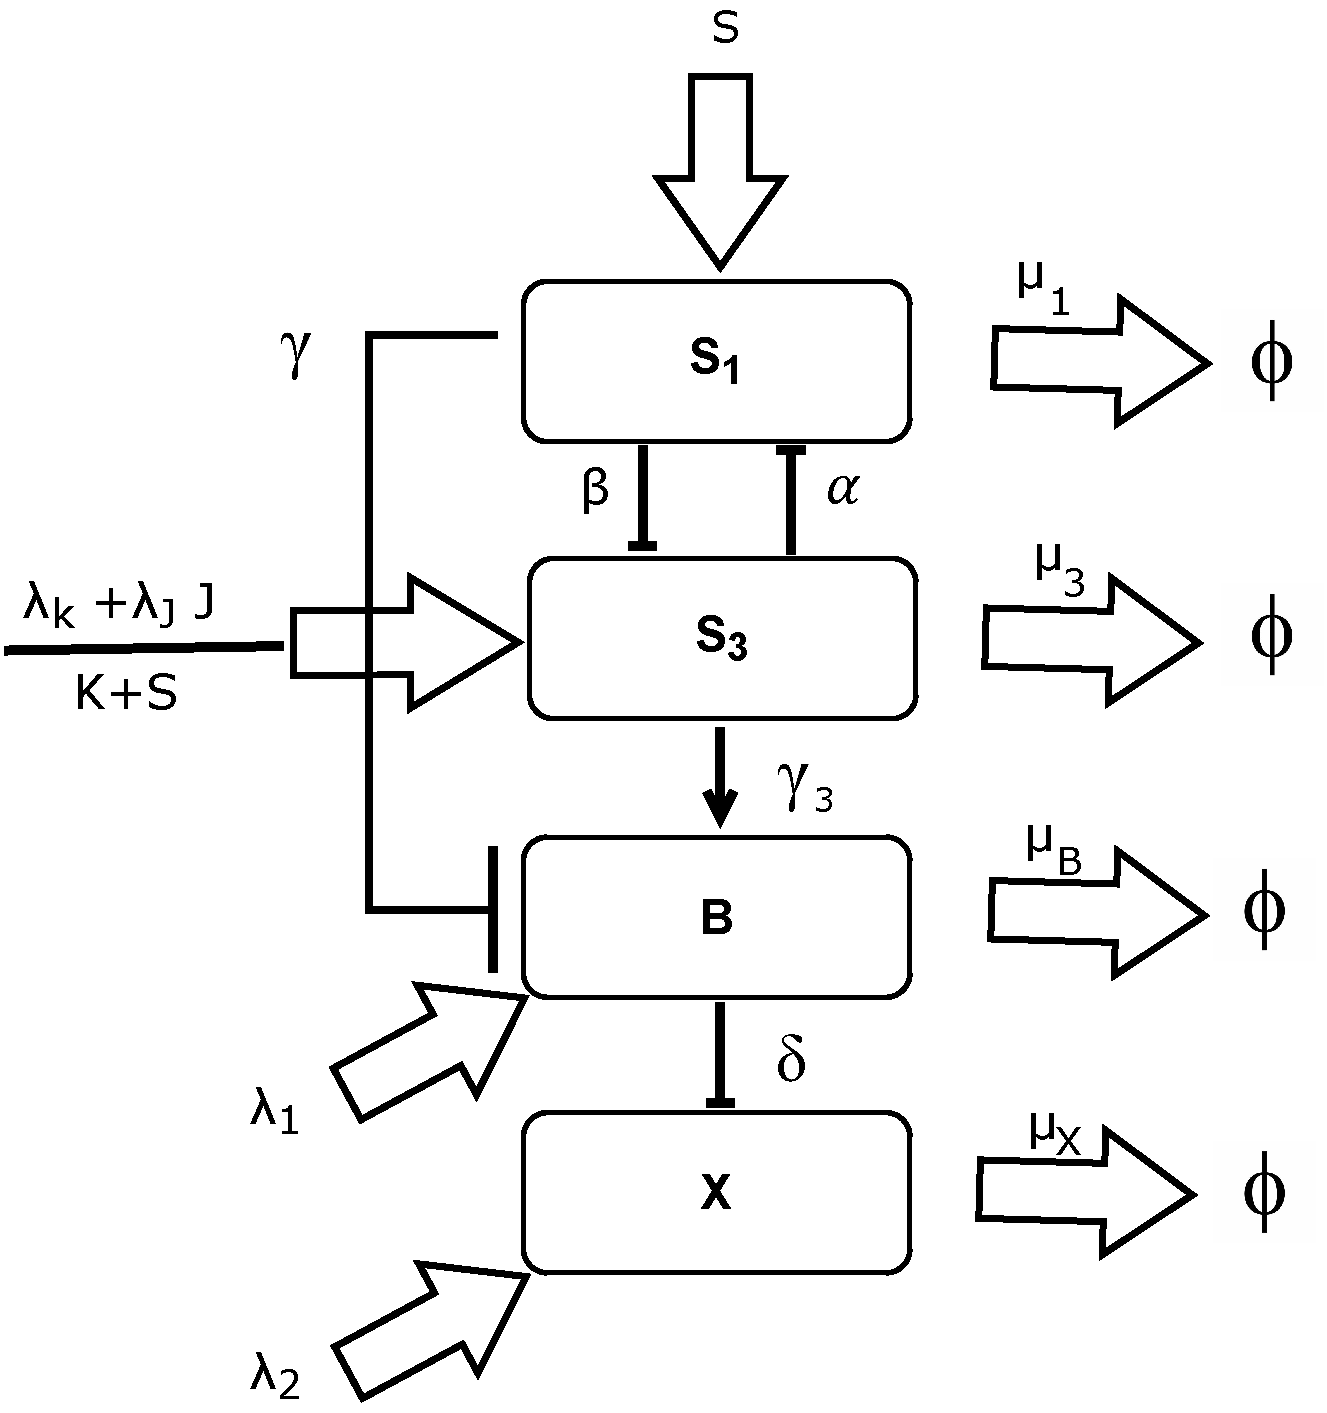
\includegraphics[width=0.7\textwidth]{Figures/D2.pdf}
		\end{framed}
	\caption{The corresponding mathematical model: levels of STAT1 and STAT3, and activity of their target Bcl2, and BAX were represented by ‘S1’, ‘S3’, ‘B’ and ‘X’, respectively \cite{lee2021mathematical}.}
	\label{D2}
\end{figure}

Figure \ref{D1} and Figure \ref{D2} is a schematic diagram that illustrates the apoptosis signalling network in response to IFN-$\beta$ and JAK2. Figure \ref{D1}, key signalling network of apoptosis: The figure illustrates the key signalling pathways involved in apoptosis, specifically the interactions between STAT1, STAT3, Bcl-2, and BAX in response to IFN-$\beta$ and JAK2. These proteins regulate the cell's response to stress, including the decision to undergo apoptosis. Figure \ref{D2},
the corresponding mathematical model: The figure also includes a mathematical representation of the signalling network. In this model, the levels of STAT1 and STAT3 are represented by 'S1' and 'S3' respectively, while the activity of their target proteins Bcl-2 and BAX are represented by 'B' and 'X' respectively. This mathematical representation mathematically models the interactions between these proteins and their responses to IFN-$\beta$ and JAK2 signalling. The model captures the dynamics of the interactions between the proteins, and allows for the prediction of the system's behavior.

Both Figure \ref{D1} and Figure \ref{D2} are representations of a mathematical model that captures the interactions of the key signalling pathways involved in apoptosis. It shows the critical signalling pathways, the proteins involved and their interactions, and the mathematical representation of the signalling network. This model allows the prediction of the system's behaviour.

\subsection{Governing ordinary differential equations (ODEs) for the intracellular signalling network}

\paragraph{}
The governing ordinary differential equations (ODEs) for the intracellular signalling network composed of STAT1, STAT3, Bcl-2, and BAX would likely be specific to the mathematical model used in a particular study. These ODEs would describe the dynamics of the concentrations of these proteins over time and would likely depend on various model parameters, such as rate constants for protein interactions and degradation.

 Let the variables $\Bar{S1}$, $\Bar{S3}$, $\Bar{B}$ and $\Bar{X}$ be concentrations of STAT1, STAT3, Bcl-2 and BAX at time $t$ respectively \cite{lee2021mathematical}. So then Then, the mass balance of the concentrations of STAT1 $\Bar{S1}$,  STAT3 $\Bar{S3}$, Bcl-2 $\Bar{B}$ and $\Bar{X}$ gives us. 

 
\begin{equation}
\label{a}
     \frac{d\Bar{S_1}}{dt} = f_{1} (s)+ \frac{ a_1a_2^2} {a_2^2+a_1F_1(\Bar{S_3})} - \mu_{s_{1}}\Bar{S_1 } 
\end{equation}

\begin{equation}
\label{b}
\frac{d\Bar{S_3}}{dt} = f_{2} (s.j)  +\frac{a_4a_5^2} {{a_5}^2+ a_6F_2({\Bar{S_3})}}-\mu_{s_{3}}\Bar{S_3} 
\end{equation}

\begin{equation}
\label{c}
\frac{d\Bar{B}}{dt} = f_3+ \frac{a_7a_8^2}{a_8^2+a_9F_3(\Bar{S_1})} -  \lambda_{STAT3} \Bar{S_3} - \mu_{Bcl2} \Bar{B} 
\end{equation}
 
\begin{equation}
\label{d}
    \frac{d \Bar{X}}{dt}= f_4 + \frac{a_10a_11^2}{a_11^2+a_12F_4(\Bar{X})} -\mu_X \Bar{X} 
\end{equation}

\newpage

The concentrations of $IFN$-$\beta$ and $JAK2$ are represented by $s$ and $j$, respectively. The rate of change in the concentration of STAT1 is determined by the input of $IFN-\beta$ through a function $f_1(s)$, the self-activating interaction with inhibition from STAT3 $(\Bar{S_3} \dashv \Bar{S_1})$ and the natural decrease in concentration at a rate $\mu_{S_1}$.  Each of ODEs equations explains the following details. 

\begin{itemize}
    \item In equation \eqref{a}, the high concentration of $IFN-\beta(s)$ upregulates the STAT1 level through the positive
function $f_1(s)$, while the high concentration of STAT3 inhibits the STAT1 level through the positive. 

\item The concentration of STAT3, represented in equation \eqref{b}, is influenced by signals from both $JAK$ and $IFN-\beta$ through a function $_2(s,j)$, self-activating interaction with inhibition from STAT1 $(\Bar{S_1} \dashv \Bar{S_3})$ and natural decrease in concentration at a rate $\mu_{S_3}$.

\item  Bcl-2 in equation \eqref{c} is regulated by the signal source at a fixed rate $f_3$, autocatalytic activity with inhibition from STAT1 $(\Bar{S_1} \dashv \Bar{B})$, upregulation from STAT3 $(\Bar{S_3} \dashv \Bar{B})$ at a rate $\lambda_{STAT3}$, and natural decay at a rate $\mu_{Bcl2}$.

\item In equation \eqref{d}, is regulated by the signal source at
a fixed rate $f_4$,  autocatalytic activity with inhibition from STAT1 $(\Bar{B} \dashv \Bar{X})$, and natural decrease in concentration at a rate $\mu_{BAX}$.
\end{itemize}

And also, we assume that, 

\begin{equation}
       f_1(s)=\lambda{IFN\beta s} , \quad    f_2(s,j)=\frac{K_2+\lambda{JAK}j}{K_1+\lambda{IFN\beta2s}}
\end{equation}

\begin{equation}
         F_1(\Bar{S_3})={\Bar{S_3}}^2 , \quad       F_2(\Bar{S_1})={\Bar{S_1}}^2, \quad  F_3(\Bar{S_1})={\Bar{S_1}}^2, \quad    F_4(\Bar{B})={\Bar{B}}^2
\end{equation}

where $\lambda_{IFN\beta}$ is the source of STAT1 from $IFN-\beta$, $\lambda_{IFN\beta2}$ is a source from $IFN-\beta$, and $\lambda_{JAK}$ is a source from JAK2. And also we use a non-dimensionalization formula as follows. 

\begin{equation}
\label{d1}
    t=\mu_{S_1}\Bar{t}, \quad     S_1=\frac{\Bar{S_1}}{{S_1}^*}, \quad S_3=\frac{\Bar{S_3}}{{S_3}^*}, \quad  B=\frac{\Bar{B}}{B^*}, \quad  X=\frac{\Bar{X}}{X^*}, \quad \mu_B=\frac{\mu_{Bcl2}}{\mu_{S_1}}, \quad \mu_X=\frac{\mu_{BAX}}{\mu_{S_1}}, \quad J=\frac{j}{J^*} \\

    k_1=\frac{a_1}{\mu_{s_1}{S_1}^*}, \quad  k_1=a_2, \quad \alpha=a_3({S_3}^*)^2, \quad  k_3=\frac{a_4}{\mu_{s_1}{S_3}^*}, \quad  k_4=a_5, \quad \beta=a_6({S_1}^*)^2, \quad \lambda_1=\frac{f_3}{\mu_{S_1}B^*} \\ 
    
    \lambda_2=\frac{f_4}{\mu_{S_1}X^*}, \quad  \lambda_k=\frac{K_2}{\mu_{S_1}{S_3}^*}, \quad \lambda_J=\frac{\lambda_{JAK}J^*}{\mu_{S_1}{S_3}*}, \quad \lambda_J=\frac{\lambda_{STAT3}{S_3}^*}{\mu_{S_1}B*}, \quad \lambda{S_1}=\frac{\lambda_{IFN\beta}S^*}{\mu_{S_1}{S_1}*}, \quad k_5=\frac{a_7}{\mu{S_1}B^*},\quad  k_2=a_2 \\
    
    k_7=\frac{a_10}{\mu{S_1}X^*}, \quad  k_6=a_8, \quad k_8=a_{11}, \quad k_4=a_5, \quad k_3=\frac{a_4}{\mu{S_1}{S_3}^*}, \quad \alpha=a_3({S_3}^*)^2, \gamma=a_9({S_1}^*)^2, \quad K=K_1\\
    
   \Lambda=a_12(X^*)^2 \quad S=\frac{s}{S^*}, \quad \beta=a_6({S_1}^*)^2, \quad \lambda_{S_2}=\lambda_{IFN\beta2}S^* \hspace{6cm}
\end{equation}


Then by using \eqref{d1} following governing equations were obtained. 

\begin{equation}
\label{e1}
     \frac{dS_1}{dt} = \lambda_{S_1} S + \frac{ k_1k_2^2} {k_2^2+\alpha S_3^2} - S_1  \\
\end{equation}

\begin{equation}
\label{e2}
\frac{dS_3}{dt} = \frac{\lambda_k+\lambda_JJ} {K+ \lambda_{S_2} S} +\frac{k_3{k_4}^2}{{k_4}^2+\beta{S_1}^2}-S_3 \\
\end{equation}

\begin{equation}
\label{e3}
\frac{dB}{dt} = \lambda_1+ \frac{k_5{k_6}^2}{{k_6}^2+\gamma{S_1}^2} -  \lambda_3 S_3 - \mu_BB \\
\end{equation}

\begin{equation}
\label{e4}
    \frac{dX}{dt}= \lambda_2+ \frac{k_7{k_8}^2}{{k_8}^2\Lambda B^2} -\mu_XX \\
\end{equation}

In the mathematical model of the kinetic network, as shown in figure 2b, the programmed cell death of cancer cells, also known as apoptosis, is triggered when the level of the anti-apoptotic protein Bcl-2 is lower than a certain threshold $(thB)$ and the level of the pro-apoptotic protein BAX is higher than another threshold $(thX)$. This is supported by experiments and previous modeling studies \cite{kim2019synergistic,bagci2006bistability,gaudette2016low}. The specific values of these thresholds were determined based on biological observations and the dynamic system of equations \eqref{e1},\eqref{e2},\eqref{e3} and \eqref{e4}.



\newpage

\section{Mathematical equilibrium and stability analysis}
\paragraph{}

The dynamics of the intracellular signalling system is governed by ordinary differential equations. 


\begin{equation}
\label{Q1}
     \frac{dS_1}{dt} = \lambda_{S_1} S + \frac{ k_1k_2^2} {k_2^2+\alpha S_3^2} - S_1  = H_1(S_1,S_3,B,X) \\
\end{equation}

\begin{equation}
\label{Q2}
\frac{dS_3}{dt} = \frac{\lambda_k+\lambda_JJ} {K+ \lambda_{S_2} S} +\frac{k_3{k_4}^2}{{k_4}^2+\beta{S_1}^2}-S_3  = H_2(S_1,S_3,B,X)\\
\end{equation}


\begin{equation}
\label{Q3}
\frac{dB}{dt} = \lambda_1+ \frac{k_5{k_6}^2}{{k_6}^2+\gamma{S_1}^2} -  \lambda_3 S_3 - \mu_BB = H_3(S_1,S_3,B,X)  \\
\end{equation}

\begin{equation}
\label{Q4}
    \frac{dX}{dt}= \lambda_2+ \frac{k_7{k_8}^2}{{k_8}^2\Lambda B^2} -\mu_XX = H_4(S_1,S_3,B,X) \\
\end{equation}

It is necessary to first identify the system's equilibrium state before exploring the equilibrium dynamics. This is accomplished by setting equations \eqref{Q1}, \eqref{Q2}, \eqref{Q3} and \eqref{Q4} to zero and performing the following calculations to find the answers $S_1^E, S_3^E, B^E$ and $X^E$:

\begin{equation}
\label{E1}
    S_1^E = \lambda_{S_1} S + \frac{ k_1k_2^2} {k_2^2+\alpha S_3^2} - S_1
\end{equation}

\begin{equation}
\label{E2}
S_3^E = \frac{\lambda_k+\lambda_JJ} {K+ \lambda_{S_2} S} +\frac{k_3{k_4}^2}{{k_4}^2+\beta{S_1}^2}-S_3  = H_2(S_1,S_3,B,X)\\
\end{equation}

\begin{equation}
\label{E3}
B^E = \lambda_1+ \frac{k_5{k_6}^2}{{k_6}^2+\gamma{S_1}^2} -  \lambda_3 S_3 - \mu_BB = H_3(S_1,S_3,B,X)  \\
\end{equation}

\begin{equation}
\label{E4}
    X^E= \lambda_2+ \frac{k_7{k_8}^2}{{k_8}^2\Lambda B^2} -\mu_XX = H_4(S_1,S_3,B,X) \\
\end{equation}
We can find the equilibrium point of the system \eqref{E1}-\eqref{E4} by nonlinear solver programming language as far as
all parameter values are fixed. 

The Jacobian matrix, J, is given by:
\begin{equation}
\label{s1}
    J = \begin{bmatrix}
\frac{\partial H1}{\partial S1} & \frac{\partial H1}{\partial S3} & \frac{\partial H1}{\partial B} & \frac{\partial H1}{\partial X} \\
\frac{\partial H2}{\partial S1} & \frac{\partial H2}{\partial S3} & \frac{\partial H2}{\partial B} & \frac{\partial H2}{\partial X} \\
\frac{\partial H3}{\partial S1} & \frac{\partial H3}{\partial S3} & \frac{\partial H3}{\partial B} & \frac{\partial H3}{\partial X} \\
\frac{\partial H4}{\partial S1} & \frac{\partial H4}{\partial S3} & \frac{\partial H4}{\partial B} & \frac{\partial H4}{\partial X}
\end{bmatrix}
\end{equation}

\begin{equation}
\label{s2}
    J = \begin{bmatrix}
-1 & -\frac{2k_1k_2^2\alpha SE_3^2}{(k_2^2 + \alpha(S_3^E)^2)^2} & 0 & 0 \\
-\frac{2k_3k_4^2\beta S_1^E}{(k_4^2+\beta(S_1^E)^2)^2} & -1 & 0 & 0 \\
-\frac{2k_5k_6^2\gamma(S_1^E)}{(k_6^2+\gamma (S_1^E)^2)} & -\lambda_3 & -\mu_B & 0 \\
0 & 0 & -\frac{2k_7k_8^2\Lambda B^E}{(k_8^2+\Lambda(B^E)^2)^2} & -\mu_X
\end{bmatrix}
\end{equation}

Then, the characteristic polynomial is given by 

\begin{equation}
\label{s3}
    (J - \Lambda I) = (\Lambda + \mu_B)(\Lambda + \mu_X) (\Lambda^2 + 2\Lambda +1 - \frac{2k_1k_2^2\alpha SE_3^2}{(k_2^2 + \alpha(S_3^E)^2)^2} \times \frac{2k_3k_4^2\beta S_1^E}{(k_4^2+\beta(S_1^E)^2)^2})
\end{equation}

Where I is the identity matrix. By using the above equations \eqref{s1}. \eqref{s2} and \eqref{s3} we can determine the stability of the system. 

 


\newpage



